\section{Introducción}\label{sec:introduccion}


% TODO: Preguntar si esto lo quiere en la presentacion o no
%\begin{frame}{Modelo}
%    \textbf{\large{Contractile Particle Model (CPM)}}
%    \begin{center}
%        \begin{minipage}[c]{0.6\textwidth}
%            \begin{block}{Características}
%                \begin{itemize}
%                    \item Las personas tienen un radio variable, $r \in [r_{min}, r_{max}]$.
%                    \item La velocidad deseada depende del radio de la persona.
%                    \item Ante el contacto, el radio de las personas se contrae al mínimo y aparece una velocidad de escape $v_e$.
%                \end{itemize}
%            \end{block}
%        \end{minipage}
%        \hfill
%        \begin{minipage}[c]{0.3\textwidth}
%            \begin{figure}
%                \centering
%                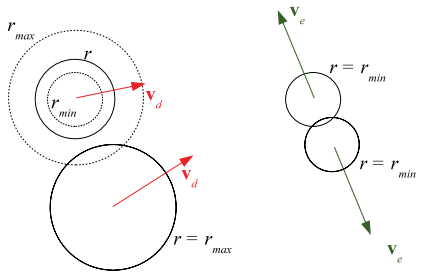
\includegraphics[width=\textwidth]{pic/01-introduccion/cpm}
%                \label{fig:cpm}
%            \end{figure}
%        \end{minipage}
%    \end{center}
%\end{frame}

\begin{frame}{Modelo operativo: Contractile Particle Model (CPM)}
    \begin{center}
        \begin{minipage}[t]{0.45\textwidth}
            \begin{block}{Rapidez deseada}
                \begin{equation*}
                    v_d^i = v_{d\ max} \left[ \frac{(r^i - r_{min})}{(r_{max} - r_{min})} \right]^{\beta}
                \end{equation*}
            \end{block}
        \end{minipage}
        \hfill
        \begin{minipage}[t]{0.45\textwidth}
            \begin{block}{Salto de instante}
                \begin{equation*}
                    \Delta t = \frac{r_{min}}{2 \max (v_{d\ max}, v_e)}
                \end{equation*}
            \end{block}
        \end{minipage}
    \end{center}
    \begin{center}
        \begin{minipage}[t]{0.45\textwidth}
            \begin{block}{Velocidad}
                \begin{equation*}
                    \mathbf{v}^i = \begin{cases}
                                       \mathbf{v}_d^i & \text{si $p^i$ está libre de contacto} \\
                                       \mathbf{v}_e^i & \text{sino}
                    \end{cases}
                \end{equation*}
            \end{block}
        \end{minipage}
        \hfill
        \begin{minipage}[t]{0.45\textwidth}
            \begin{block}{Salto de radio}
                \begin{equation*}
                    \Delta r = \frac{r_{max}}{\left( \frac{\tau}{\Delta t} \right)}
                \end{equation*}
            \end{block}
        \end{minipage}
    \end{center}
\end{frame}

\begin{frame}{Heurísticas}
    \begin{block}{Defensores}
        \footnotesize{\text{Su dirección objetivo es la posición del atacante.}}
        \begin{equation*}
            \mathbf{n}_{desired}^{def\ j} = \mathbf{x}_{at} - \mathbf{x}_{def\ j}
        \end{equation*}
    \end{block}
    \begin{block}{Atacante}
        \footnotesize{
            \text{Determinada por CPM modificado, ya que debe llegar a su posición objetivo principal, el \textit{in-goal} izquierdo,}
            \text{y al mismo tiempo evitar a los defensores.}
        }
        \begin{minipage}{0.75\linewidth}
            \begin{equation*}
                \begin{aligned}
                    \mathbf{n_c}_{def\ j}^{at} &= A_p\ e^{-\frac{d_{at,def\ j}}{B_p}} &&& \mathbf{n_c}^{at} &= \sum_{j=1}^{N_j} \mathbf{n_c}_{def\ j}^{at} \\
                    \mathbf{e}_{target}^{at} &= \frac{\mathbf{x}_{goal} - \mathbf{x}_{at}}{\left\| \mathbf{x}_{goal} - \mathbf{x}_{at} \right\|} &&& \mathbf{n}_{desired}^{at} &= \mathbf{n_c}^{at} + \mathbf{e}_{target}^{at}
                \end{aligned}
            \end{equation*}
        \end{minipage}
        \begin{minipage}{0.2\linewidth}
            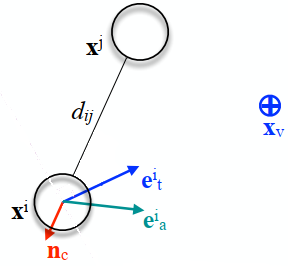
\includegraphics[width=\textwidth]{pic/01-introduccion/cpm-modified}
        \end{minipage}
    \end{block}
\end{frame}

\begin{frame}{Heurísticas}
    \begin{block}{Velocidad deseada}
        \text{Para todo jugador, la velocidad deseada se define}
        \begin{equation*}
            \begin{aligned}
                \mathbf{e}_{desired}^i &= \frac{\mathbf{n}_{desired}^i}{\left\| \mathbf{n}_{desired}^i \right\|} \\
                \mathbf{v}_{d}^i &= v_{d\ max}\ \mathbf{e}_{desired}^i
            \end{aligned}
        \end{equation*}
    \end{block}
\end{frame}




